%!TEX root = ../../root.tex

\emph{Dropout} provides a computationally inexpensive but
powerful method of regularizing a broad family of models. 
To a first approximation, dropout can be thought of as a method of making bagging practical for \emph{ensembles} of very many large neural networks.

Assume you have unlimited computational power. It would be possible to generate thousands  of deep networks, train all of them on the same data and then take the average prediction as final prediction. In machine learning this way of proceeding is called \emph{ensemble} machine learning. Ensemble predictions (e.g. bayesian networks, random forests) are known to generalize better than the individual models.

Given a multi-layer perceptron network, we could generate an ensemble of deep neural networks by randomly removing some of the nodes. This will result in a different network and therefore will represent a different function. 
Dropout can be considered an ensemble method for deep learning, which 
parametrizes each model in the ensemble by \emph{dropping} random units (i.e. nodes with their input/output connections) of the ``main'' network.
\begin{figure}[H]
    \centering
    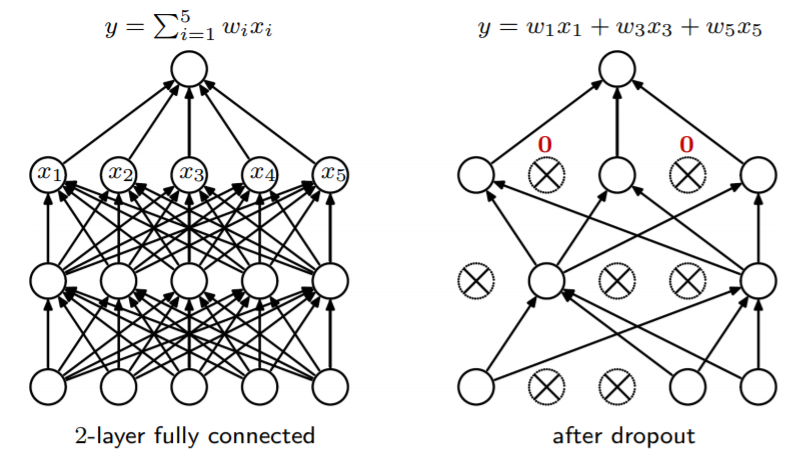
\includegraphics[width=.8\textwidth]{09/21_27}
    \caption{Before and after dropout.}	
\end{figure}

\paragraph{Implicit ensembles}
Dropout has two distinguishing features:
\begin{itemize}
    \item It does \emph{bagging}: for a family of models, each model is trained on a subset of the data (e.g. mini-batches).
    \item It does \emph{weight sharing}, which is \emph{atypical} in ensemble methods.
\end{itemize}

In fact, since we do not have unlimited computational power and thus it would be infeasible to \emph{explicitly} generate an ensemble of different configurations, dropout \emph{implicitly} defines the ensemble keeping just \emph{one single network} and randomly removing (zero-out) some of its units, each with a specified probability $p$ of being retained, chosen by the user, globally for the whole network or also \emph{per layer}.
\\

\textbf{Note.} How large would an explicit ensemble built from sampling the network be? If the network contains $n$ units, then each sampled network can either be present in the network or not, so we have $2^n$ possible configurations.

\subparagraph{Training} 

At training time, dropout generates a new sampling of the network each time new training data is presented (e.g. \emph{at each mini-batch} in SGD), that thus enters a completely new configuration of the network.

The individual models (samples of the original network) are \emph{not} optimized to convergence because they are ``discarded'' in favor of new, different models at each optimization step. 

However, the \emph{ensemble} is trained to convergence: at each training step the weight update is applied to all members of the ensemble (i.e. the original network) simultaneously.

\begin{figure}[H]
    \centering
    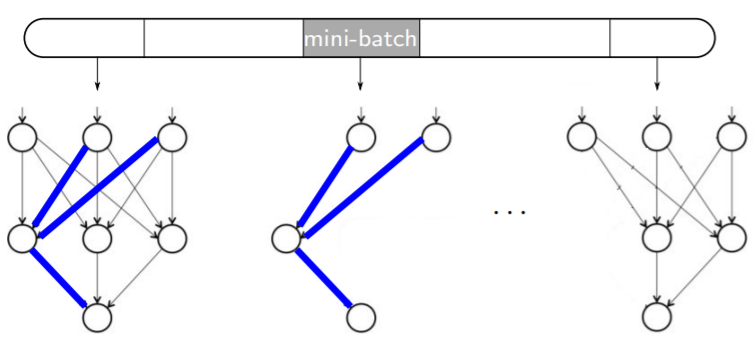
\includegraphics[width=.5\textwidth]{09/23_27}
    \caption{New models are generated one by one as one produces new mini-batches during optimization. Notice the weight sharing, e.g. the blue edges have the same weights in every model that contains them.}	
\end{figure}
    
\subparagraph{Testing}

At test time ensembles typically produce their output as some form of \emph{average} of the output of all their members. 
Since in the case of dropout the members are defined only implicitly, the trained weights from each model in the ensemble must be \emph{averaged} somehow. The simple idea is that if a unit is retained with probability $p$ during training, its outgoing weights are multiplied by $p$, since the average contribution of that unit in training the ensemble has been $p$.
\begin{figure}[H]
    \centering
    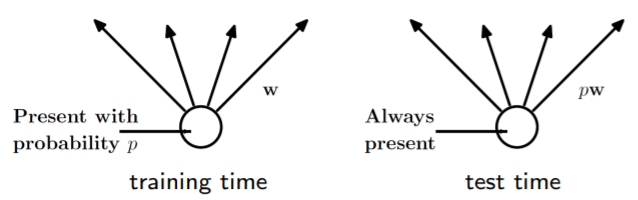
\includegraphics[width=.5\textwidth]{09/22_27}
    \caption{Dropout: training time vs test time.}	
\end{figure}

\paragraph{Properties as a regularizer}

In a standard neural network, weights are optimized \emph{jointly}. This
means that errors in the optimization are spread across all the weights. If 
a unit in the neural network is making mistakes (e.g. has learnt a sub-optimal hidden representation) then probably there will be some later unit in the network making up for it. Units are allowed to do mistakes because these mistakes will be absorbed by some other unit. This is called \emph{co-adaptation} in the literature. 

Although it may seem like a nice failsafe, it is actually something we want to avoid because it worsen the \emph{transferabilty} of the network to unseen new data.
\begin{itemize}
    \item Dropout \emph{reduces} co-adaptation by making units unreliable (they can appear and disappear suddenly, so earlier units that relied on later units to correct their mistakes are discouraged to do so). 
    This improves \emph{generalization} to unseen data, and reduces overfitting.
    
    \item Dropout learns \emph{sparse} representations, meaning that the intermediate variables will tend to be sparse. This is a nice side-effect that has been observed in practice, since dropout is not explicitly designed to do so.
    
    \item Performs closely to \emph{exact} model averaging over all $2^n$ models 
    and much better if no weight sharing is done in the exact model.
    
    \item \emph{Longer} training times (usually $2$ to $3$ times longer), since parameter updates are now noisier.
    Dropout is another source of stochasticity in addition to the mini-batches.
    
    \item Typical choices: $20$\% of the input units and $50$\% of the hidden units.
\end{itemize}

\begin{figure}[H]
    \centering
    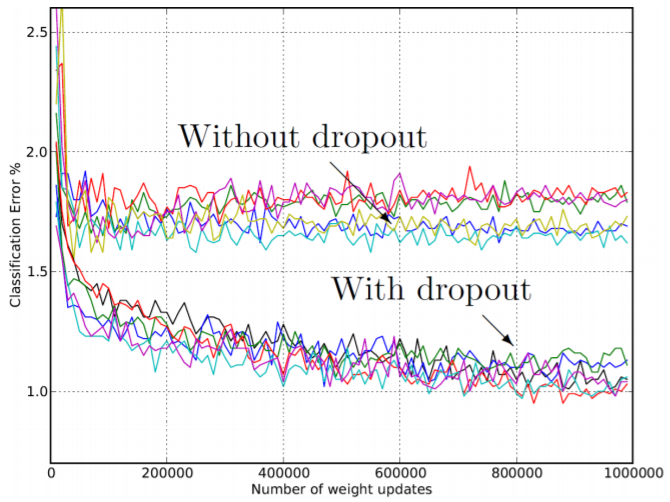
\includegraphics[width=.5\textwidth]{09/25_27}
    \caption{Validation error comparison.}	
\end{figure}

\subparagraph{Dropout as an explicit penalty}

It has been shown that in a $2$-layer network 
\begin{equation}
    \vb{\hat{y}} = \sigma(\vb{V}(\sigma(\vb{U} \vb{x})))
\end{equation}
applying dropout is formally equivalent to changing the loss function by including the following weight penalty:
\begin{equation}
    \ell(\mathbf{U},\mathbf{V}) + \frac{1-p}{p} \sum_{i=1}^r \| \mathbf{u}_i\|^2 \| \mathbf{v}_i\|^2
\end{equation}
where the vectors are the columns of $\mathbf{U}$ and $\mathbf{V}$. This is a form of \emph{path regularizer}, since it computes a sum of products of squared weights along each possible path from input to output. 

This regularizer term tends, at the optimum, to equalize the norms $\| \mathbf{u}_i\|^2,\| \mathbf{v}_i\|^2$ for all $i$, which is conjectured to reduce co-adaptation since it is equalizing the contribution of each unit. For a small enough dropout rate, it can be shown that all minima are \emph{global}.

In practice this is not very useful to us, but it is interesting to appreciate how an implicit regularizer such as dropout can be turned into an explicit penalty expression.